
\chapter{技术方案}\label{chapter_system}
本章将介绍安卓控件检测内存泄露的原理。首先将从宏观上对安卓不可见控件内存泄漏的自动化检测工具进行全面的讲述,提出测试的主要流程和步骤。接下来在后续的章节中对各个模块进行具体的细节讲述。

\section{系统架构}


首先,测试的资料为由其他开发者所开发的\textbf{.apk}文件,本文的测试对象是服务和广播接收器,但是我们不可能阅读应用的源码。如前文中对服务和广播接收器的描述,我们需要寻找合适的工具对apk文件进行解析反编译,目的是得到\textbf{AndroidManifest.xml}清单文件,接下来编写脚本对该清单进行解析,从而得到本文关注的测试对象(公开服务和清单中注册的静态广播接收器),生成一份测试配置。

然后,为了实现安卓系统上的\textbf{跨应用组件}的测试,需要设计实现一个安卓应用,这个安卓应用的作用是驱动整个在安卓系统上的测试步骤,例如:读取测试配置,进行跨应用组件的启动与关闭,处理测试时发生的异常(Exception)等等。后文将称此应用为\textbf{测试驱动应用}。

接下来,当测试完成时,我们需要判定被测试应用是否发生了内存泄露,所以必须要将被测试应用的堆内存镜像拷贝导出,然后对这一时刻的堆中的对象设计算法进行分析,从而得出测试结果。后文将称此分析工具为\textbf{内存分析器}。

\subsection{基于测试效率的考量}

由于测试时,必然要启动安卓模拟器,而安卓模拟器的运行原理为虚拟机,将会占用固定数额的电脑内存等资源,因此如果所有步骤都在安卓模拟器上完成将会使效率大打折扣。

结合上文的方案概述,可以将若干与主要测试流程不相关、或者安卓模拟器上很难实现的步骤放到工作站上来进行,即解析apk文件和内存分析。

因此需要建立安卓模拟器和工作站的通讯,由于通讯功能在本文中只需要很少的功能,因此可以使用python建立简单的socket连接即可。

\subsection{具体设计}
\begin{figure}[htbp]
	\centering
	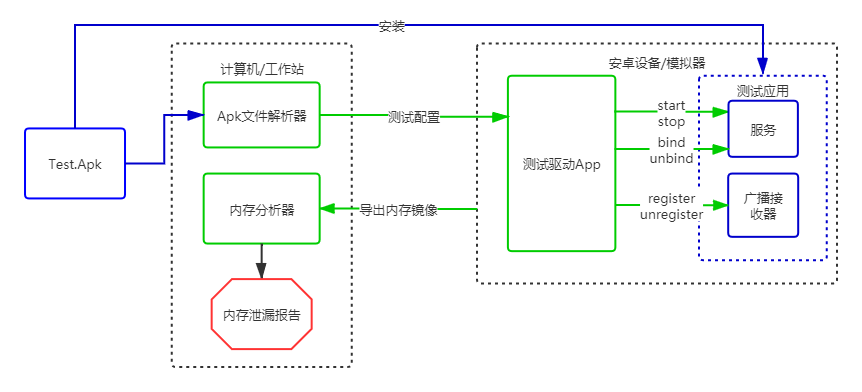
\includegraphics[width=0.9\textwidth]{main_flow.png} % requires the graphicx package
	\caption{自动检测工具原理}
	\label{fig:flow}
\end{figure}

如图\textbf{\textcolor{red}{\ref{fig:flow}}}所示,测试将在两个环境(工作站、安卓模拟器)中完成:
\begin{enumerate}
	\item 在工作站中,使用\textbf{Apk文件解析器}(详见\textbf{\textcolor{red}{\ref{apk analyser}}})对被测试应用\textbf{Test.apk}进行反编译,并解析\textbf{AndroidManifest.xml}清单,得到在清单中注册的\textbf{公开服务}以及\textbf{清单声明的广播接收器},作为测试对象生成一份\textbf{测试配置}发送到安卓模拟器上。
	\item 在安卓模拟器上安装好\textbf{测试驱动App}(详见\redbf{\ref{test driver app}})以及被测试应用\textbf{Test.apk}。通过\textbf{ADB}向安卓模拟器发送指令启动\textbf{测试驱动App},它会读取步骤1中发送来的\textbf{测试配置},然后执行测试主流程(详见\redbf{\ref{main flow}})
	\item 在完成测试主流程之后,通知工作站将被测试应用的堆镜像文件(.prof)文件导出,使用\textbf{内存分析器}(详见\redbf{\ref{memory analyser}})进行内存泄漏的检测,最终生成一份\textbf{内存泄漏报告}显示被测试应用的服务以及广播接收器有无内存泄漏情况,以及具体的内存泄漏的控件清单。
\end{enumerate}

\section{Apk 文件解析器}\label{apk analyser}
Apk 文件解析器旨在通过将被测试应用反编译得到\textbf{AndroidManifest.xml}清单,对该清单进行分析,从而得到在清单中声明的\textbf{公开服务}以及\textbf{广播接收器}作为测试对象。
\begin{listing}[htbp]
	\centering
	\caption{使用apktool工具进行apk的反编译}
	\begin{minted}[encoding=utf8,
	frame=single,
	framesep = 1em,
	numbers=left, 
	breaklines=true, 
	tabsize=4,
	showtabs = false,
	xleftmargin=2em,xrightmargin=2em,
	fontsize=\footnotesize]{shell}
apktool d -f $test_apk$ -o temp
	\end{minted}
	\label{shell:apktool}
\end{listing}

使用apktool工具\cite{apktool},执行\textbf{Listing.}\redbf{\ref{shell:apktool}}中的命令即可完成被测试应用的反编译得到\textbf{AndroidManifest.xml}清单。

\begin{listing}[htbp]
	\centering
	\caption{使用python解析xml输出测试配置}
	\begin{minted}[encoding=utf8,
	frame=single,
	framesep = 1em,
	numbers=left, 
	breaklines=true, 
	tabsize=4,
	showtabs = false,
	xleftmargin=2em,xrightmargin=2em,
	fontsize=\footnotesize]{python}
from xml.dom.minidom import parse
def get_exported_services(xml_path):
	exported_services = []
	manifest = parse(xml_path).documentElement 
	for service in manifest.getElementsByTagName('service'):
		exported = service.getAttribute('android:exported')
		enabled = service.getAttribute('android:enabled')
		if (exported == 'true' and (enabled == '' or enabled == 'true')):
			exported_services.append(service)
	return exported_services
	
def get_static_receivers(xml_path):
	exported_receivers = []
	domTree = parse(xml_path)
	manifest = domTree.documentElement
	for receiver in manifest.getElementsByTagName('receiver'):
		enabled = receiver.getAttribute('android:enabled')
		if (enabled == '' or enabled == 'true'):
			exported_receivers.append(receiver)
	return exported_receivers;
	\end{minted}
	\label{python:get services}	
\end{listing}

接下来使用\textbf{python}中的\textbf{xml} 库解析此xml文件(详见\textbf{Listing.}\redbf{\ref{python:get services}}),筛选出所有指定\textbf{android:exported = "true"} 以及 \textbf{android:enabled = "true"}(或者不指定,默认值为"true")的服务,以及在清单中声明的广播接收器。将这些控件的包名,类名,以及所需的权限等信息写入\textbf{测试配置}中
\section{测试驱动App}\label{test driver app}
测试驱动App负责控制所有安卓模拟器上的测试行为(即测试主流程\redbf{\ref{main flow}})。首先驱动会读取\textbf{测试配置},获得要测试的服务和广播接收器,之后进行\textbf{测试主流程},在完成测试流程之后,使用\textbf{Socket}与\textbf{工作站}进行通信,通知\textbf{工作站}测试任务已经完成,导出被测试应用的堆镜像文件进行最后的分析。
\section{测试主流程}\label{main flow}

\begin{algorithm}
	\caption{测试主流程:公开服务测试}
	\label{alg:service}
	\begin{algorithmic}[1]
		\STATE {读取测试配置}
		\FOR{遍历测试配置中的公开服务}
			\STATE{重置安卓模拟器}
			\STATE{重置计数器}
			\IF{使用bind方式测试}
				\STATE{启动仿真Activity}
			\ENDIF
			\WHILE{计时器 < 测试重复次数}
				\IF{使用start方式测试}
					\STATE {调用startService() API 启动服务} 
					\STATE {调用stopService() API 停止服务}
				\ELSE
					\STATE{调用bindService() API 将服务绑定到Activity上}
					\STATE{调用unbindService() API 解除服务绑定}
				\ENDIF
				\STATE{计数器自增1}
			\ENDWHILE
			\IF{使用bind方式测试}
				\STATE{销毁仿真Activity}
			\ENDIF
			\STATE{通知工作站导出堆镜像}
		\ENDFOR
	\end{algorithmic}
\end{algorithm}

\begin{algorithm}
	\caption{测试主流程:清单声明的广播接收器}
	\label{alg:receiver}
	\begin{algorithmic}[1]
		\STATE {读取测试配置}
		\FOR{遍历测试配置中的广播接收器}
			\STATE{重置安卓模拟器}
			\STATE{重置计数器}
			\WHILE{计时器 < 测试重复次数}
				\STATE{构造特定广播,定向发送给该接收器}
				\STATE{计数器自增1}
			\ENDWHILE
			\STATE{通知工作站导出堆镜像}
		\ENDFOR
	\end{algorithmic}
\end{algorithm}

在测试主流程中,对服务和接收器进行逐一测试:

\textbf{服务测试(见算法\redbf{\ref{alg:service}}) }  测试原理为对被测试应用进行大量重复的启动和关闭(根据测试要求不同分为start/bind 和stop/unbind),确保潜在的内存泄漏被触发,之后将被测试应用的堆镜像导出,送入\textbf{内存分析器}(详见\redbf{\ref{memory analyser}})进行检测和分析。

\textbf{广播接收器测试(见算法\redbf{\ref{alg:receiver}}) }
广播接收器的测试不需要事先启动应用,因为在清单中注册的广播接收器在应用安装时就会在系统中进行注册,在任何时候都可以接收广播(即使应用未运行),因此只需要构造接收器订阅的广播,定向发送给该接收器就可以触发该接收器。同样的为了确保潜在的内存泄漏被触发,需要重复发送大量的广播。最终将被测试应用的堆镜像导出,送入\textbf{内存分析器}(详见\redbf{\ref{memory analyser}})进行检测和分析。
\section{内存分析器}\label{memory analyser}

\begin{algorithm}
	\caption{内存分析器:服务分析}
	\label{alg:memory analyser:service}
	\begin{algorithmic}[1]
		\STATE{导入并解析.hprof文件}
		\STATE{查询所有Service的衍生类集合}
		\FOR {遍历Service的衍生类集合}
			\IF{该实例已经被销毁}
				\STATE{获得所有该实例到GC Root的路径集合}
				\STATE{去除路径集合中不合理的路径}
				\IF[证明该实例确实已经被销毁]{路径集合为空}
					\STATE{该实例不存在内存泄漏}
				\ELSE[该实例仍然被引用,产生内存泄漏]
					\STATE{该实例产生内存泄漏}
					\IF{该实例内存泄漏原因为已知的安卓系统BUG}
						\STATE{不判定构成人为内存泄漏}
					\ELSE
						\STATE{由开发者构成的人为内存泄漏}
					\ENDIF
				\ENDIF
			\ENDIF
		\ENDFOR
	\end{algorithmic}
\end{algorithm}

\begin{algorithm}
	\caption{内存分析器:服务分析}
	\label{alg:memory analyser:receiver}
	\begin{algorithmic}[1]
		\STATE{导入并解析.hprof文件}
		\STATE{查询所有BroadcastReciver的衍生类集合}
		\FOR {遍历BroadcastReceiver的衍生类集合}
			\IF{该实例已经被销毁}
				\STATE{获得所有该实例到GC Root的路径集合}
				\STATE{去除路径集合中不合理的路径}
				\IF[证明该实例确实已经被销毁]{路径集合为空}
					\STATE{该实例不存在内存泄漏}
				\ELSE[该实例仍然被引用,产生内存泄漏]
					\STATE{该实例产生内存泄漏}
					\IF{该实例内存泄漏原因为已知的安卓系统BUG}
						\STATE{不判定构成人为内存泄漏}
					\ELSE
						\STATE{由开发者构成的人为内存泄漏}
					\ENDIF
				\ENDIF
			\ENDIF
		\ENDFOR
	\end{algorithmic}
\end{algorithm}

内存分析器负责从堆镜像文件(\textbf{.hprof文件})中识别和统计服务(广播接收器)的内存泄漏实例,基于开源工具MAT\cite{mat}进行定制化的开发,具体原理(详见\textbf{算法\redbf{\ref{alg:memory analyser:service}}及\redbf{\ref{alg:memory analyser:receiver}}})为:首先导入并解析堆镜像文件,找到所有的服务(广播接收器)实例,接下来对于每个找到的实例,逐个检测判断是否产生了内存泄露,对于产生内存泄漏的控件,生成一份内存泄漏分析报告。

\textbf{服务的内存泄露判定 } 所有仍然活跃的服务都会被\textbf{ActivityThread} 的 \textbf{mServices}变量所引用,而所有被销毁的服务都会被从\textbf{mServices}中删除。一个对象的实例如果实际上处于存活状态,则一定会拥有至少一条有效的\textbf{GC Root Path}。因此服务内存泄漏的判定充要条件为:拥有至少一条有效的\textbf{GC Root Path}且不在\textbf{mServices}中。

\textbf{广播接收器的内存泄漏判定 } 由于广播接收器被系统规定为不耗时控件(超过10s未完成\textbf{onReceive()} 方法,将会抛出\textbf{ANR Exception}导致应用崩溃),因此对于广播接收器而言,只需要检测是否有实际处于存活状态的实例即可。即:拥有至少一条有效的\textbf{GC Root Path}。

\textbf{安卓系统自身原因产生内存泄漏 } 由于安卓系统自身可能存在\textbf{BUG}导致正常的控件产生内存泄漏,此类问题并非由于安卓应用开发者的失误而导致,因此要将此类内存泄漏排除。

\section{其他实现细节}

\textbf{后台服务限制 }\cite{android-service-limit} 在安卓8中,新增了“电池优化策略”,系统不允许后台应用创建后台服务,因此跨应用对服务进行测试将会失败。解决办法为:禁用系统的电池管理服务;在测试时,将被测试应用置于前台。

\textbf{广播限制 }\cite{android-receiver-limit} 在\textbf{安卓8}及更高版本系统的应用中禁止将隐式广播注册为清单声明的广播接收器。而显示广播和需要签名授权的广播接收器不受限制,可以继续注册为清单声明的广播接收器。\textbf{注意:}随着安卓系统的更新,很多隐式广播已经不再受到此规定的限制,具体的广播列表可以参考隐式广播例外\cite{android-receiver-limit-exception}。

\textbf{超级用户限制 } 在\textbf{安卓7}以及更早的版本中,开发者经常会将系统增加超级用户权限,以便于进行测试(亦成为\textbf{root}),大致的方法为将兼容的二进制文件\textbf{su}拷贝到安卓设备中,使安卓设备可以执行超级用户指令\textbf{sudo},进而为测试带来便利。然而再\textbf{安卓8}以及更高的系统中,由于用于\textbf{root}操作的二进制文件\textbf{su}维护团队相继解散,获得非安卓系统开发人员获得超级用户权限变得困难,因此本文的自动化检测工具的实现不要求对系统进行\textbf{root},而将使用\textbf{socket}建立安卓设备与工作站的通信,由工作站使用\textbf{adb}指令完成跨应用的特殊权限操作:比如\textbf{跨应用导出堆镜像文件}操作需要应用拥有超级用户权限,而使用\textbf{adb}指令则不需要超级用户权限即可导出任意应用的堆镜像文件。
\newline
\section{小结}
本章中主要讨论了自动化检测工具实现的流程、细节以及若干基于测试效率的考量,然后说明了各个模块的实现细节,以及各种检测分析的算法原理。最后说明了一些方案不可行的原因。